\chapter{Experimentos e resultados}\label{experimentos}

Neste capítulo serão apresentados os experimentos feitos durante o TCC. Eles tiveram como
finalidade avaliar o uso de métodos e técnica de compressão de modelos, focado em dispositivos
embarcados. Nele serão apresentados o dispositivo utilizado (\autoref{sec_dispositivo}),
modelos usados (\autoref{sec_modelo_utilizado}), métodos de treinamento (\autoref{sec_treinamento_modelo}),
o método de avaliação do modelo (\autoref{sec_avaliacao_modelo}), \textit{datasets} utilizados
(\autoref{sec_datasets}) e resultados (\autoref{sec_resultados}).

\section{Dispositivo utilizado}\label{sec_dispositivo}
% Para avaliar os modelos, foram usados diversos dispositivos para que seja possível medir a sua performance em mais de um
% ambiente.
%
% \subsection{Desktop}\label{sec_dispositivo_desktop}
% Para auxiliar na etapa de avaliação dos modelos, foi utilizado um computador com o processo AMD Ryzen 5 4600G e 16GB de
% memória ram, ele serviu como base para avaliação por ser um dispositivo com grande poder computacional.
%
% Além disso, ele foi o ambiente de desenvolvimento do projeto, onde foram desenvolvidos os benchmarks e utilitários
% usados no trabalho.
%
% \subsection{ESP32-S3}\label{sec_dispositivo_esp}
O ESP32-S3 N16R8 foi escolhido pelo seu custo-benefício, sendo um aparelho poderoso considerando o seu baixo
custo e consumo energético. Além disso, esse dispositivo possui um processador 32-bit Xtensa dual-core,
16 MB de memória flash e 8 MB de PSRAM, permitindo que modelos maiores sejam portados para esse dispositivo sem redução
% NOTE: Rever
de parâmetros, podendo afetar o tempo de inferência do modelo.

Para executar os modelos no ESP foi utilizado o projeto person-detection do repositório esp-tflite-micro da Espressif
\footnote{Disponível em: \url{https://github.com/espressif/esp-tflite-micro/tree/master} Acessado em Março de 2025}.
A partir desse projeto, os modelos foram portados, sendo necessário realizar algumas alterações no projeto,
para suportar o tamanho dos modelos e suas camadas, e adicionar alguns utilitários, como um \textit{log} com
o uso da memória.

\section{Modelos utilizados}\label{sec_modelo_utilizado}
Para realizar os experimentos, os modelos \textbf{MobileFaceNet}, \textbf{Rafael-2} e \textbf{MobileNetV3Small}
foram utilizados como teste, tanto na etapa de treinamento (\autoref{sec_treinamento_modelo}) quanto de avaliação
(\autoref{sec_avaliacao_modelo}).

Para treinar os modelos, foi utilizada a plataforma kaggle\footnote{
Disponível em: \url{https://www.kaggle.com/}. Acessado em Março de 2025}, o \textit{dataset} utilizado foi
\textit{Labeled Faces in the Wild} (LFW) \footnote{
Disponível em: \url{https://www.kaggle.com/datasets/luhtookyaw/lfwpreparedtriplets}. Acessado em Março de 2025.},
onde os métodos de treinamento \textit{Triplet Loss} e \textit{Triplet Distillation}
\cite{triplet_distillation_face_recognition} foram utilizados, pois são eficazes para melhorar a precisão do modelo,
no contexto de reconhecimento facial.
Além disso os modelos foram treinados considerando com imagens R8G8B8, assim reduzindo a quantidade de memória necessária
para carregar as imagens no ESP32-S3, onde cada imagem tem seus pixels representados por triplas de 8 bits, contendo o
valor das cores vermelho, verde e azul, respectivamente.

% TODO: Ver se eu posso deixar esse footnote
Para validar os resultados de cada modelo, foi criado o repositório model-eval\footnote{
Disponível em: \url{https://github.com/LuanFabricio/model-eval}. Acessado em Março 2025.}, para ser utilizado junto com o
\textit{dataset} Faces - UFS \cite{leandro}.
Onde o método de validação consiste em comparar uma imagem com \textit{flip} com todo o \textit{dataset}, e definindo
a classe prevista pelo modelo aquela que possui menor distância de cosseno.
% \subsection{MobileFaceNet}
% O modelo utilizado foi o MobileFaceNet, pois ele mantém uma acurácia acima de 90\% na tarefa de detecção de faces,
% com tempo de inferência e baixa pegada de memória \cite{leandro}.

MobileFaceNet é um modelo focado para fazer reconhecimento de faces em tempo real em dispositivos móveis,
assim possuindo uma baixa pegada de memória, abaixo de 5MB e mantendo uma acurácia alta, acima de 90\% \cite{leandro}.

% \subsection{Rafael-2}
Rafael-2 é uma variação do modelo Rafael \cite{rafael}, adaptada para realizar a tarefa de reconhecimento facial.
Como o modelo base é simples e focado para dispositivos embarcados, ele possuí uma baixa quantidade de parâmetros,
 o que melhora a performance do modelo em dispositivos embarcados.

% \subsection{MobileNetV3Small}
MobileNetV3Small é uma variação do MobileNetV3, com uma quantidade reduzida de parâmetros, reduzindo a sua pegada de
memória e aumentando a performance.
% TODO: CITAR ARTIGOS

% ADICIONAR TABELA COM O CONSUMO DE RECURSOS DO MODELO
\begin{table}[htb]
\centering
\ABNTEXfontereduzida
\caption[Recurso utilizado por modelo]{Recurso ocupado pelos modelos utilizados}
\label{tabela_modelos}
\begin{tabular}{ |c|c|c|c|c| }
	\hline
	\textbf{Modelo} 	& \textbf{Quantização} & \textbf{Quantidade de Parâmetros} & \textbf{Tamanho do arquivo (TFLite)} \\
	\hline
	MobileFaceNet 		& - 	& 1.154.065 & 4.5MB \\
	MobileFaceNet 		& uint8 & 1.154.065 & 1.5MB \\
	Rafael-2 		& - 	& 351.522  & 1.4MB \\
	Rafael-2 		& uint8 & 351.522   & 356KB \\
	MobileNetV3Small 	& - 	& 1.088.357 & 1.4MB \\
	\hline
\end{tabular}
\legend{Fonte: Autor}
\end{table}

Na \autoref{tabela_modelos}, é possível observar o parâmetros e pegada de memória dos modelos, com base na quantização
utilizada.
Com isso, é possível perceber que o modelo mais simples, menor quantidade de parâmetros e que necessita de menos recurso
é o Rafael-2, enquanto o mais complexo, com maior quantidade de parâmetros e que necessita de mais recurso é o
MobileFaceNet. Também, é válido destacar que as suas versões quantizadas reduziram consideravelmente a quantidade de
memória utilizada pelos modelos.

\section{Método de treinamento do modelo}\label{sec_treinamento_modelo}
Para fazer o treinamento dos modelos, foi necessário utilizar a técnica de \textit{Triplet Distillation}
\cite{triplet_distillation_face_recognition},
para que seja possível medir o quão próximo as \textit{embeddings} de uma imagem são parecidas com as de outra.
Essa técnica usa três imagens: \textbf{âncora}, que é serve como imagem base; \textbf{positiva},
que é uma variação da mesma categoria da \textbf{âncora}; e a \textbf{negativa}, que pertence a outra categoria.

No contexto de reconhecimento facial, os \textit{embeddings} das imagens \textbf{âncora} e \textbf{positivas}
devem possuir uma distância de cosseno pequena, enquanto o vetor de característica das imagens
\textbf{âncoras} e \textbf{negativas} devem possuir uma distância de cosseno alta.

\subsection{\textit{Triplet Loss}}
Para realizar o treinamento do modelo MobileFaceNet, foi utilizada a técnica \textit{triplet loss}
\cite{triplet_distillation_face_recognition}. Ela tem como objetivo comparar os \textit{embeddings} de três imagens,
utilizando a distância de cosseno ($D$) de um embedding ($x_i^j$) comparado com outro ($x_i^k$).
%Essa técnica utiliza é descrita pela fórmula \ref{eq_triplet_loss}

\begin{equation}\label{eq_triplet_loss}
	Loss = \frac 1 N \sum _i ^N max(D(x_i^a, x_i^p) - D(x_i^a, x_i^n) + m, 0))
\end{equation}
%
% \begin{equation}\label{eq_triplet_loss_teacher_dist}
% 	d = max(T(x_i^a, x_i^n) - T(x_i^a, x_i^p), 0)
% \end{equation}
%

Na equação \ref{eq_triplet_loss}, é a função \textit{Loss} utilizada para treinar o modelo. Onde, $x_i^a$ é
a imagem âncora, $x_i^p$ é a imagem positiva e $x_i^n$ é a imagem negativa, todas referentes a i-ésima
tripla e $m$ é um hiperparâmetro que define a margem entre o par positivo e par negativo.
Então, quanto mais parecidos forem os \textit{embeddings} da imagem âncora com a imagem positiva,
menor será a perda, sendo o inverso para a âncora com a imagem negativa.

\subsection{\textit{Triplet Distillation}}
Para realizar o treinamento dos modelos MobileNetV3 e Rafael-2, foi utilizada a técnica de
\textit{Knowledge Distillation} \cite{hinton2015distilling} com \textit{Triplet Loss}, conhecida como
\textit{triplet loss} \cite{triplet_distillation_face_recognition}.
Ela utiliza cálculo da \textit{Loss Function} (\ref{eq_triplet_loss}) como base, adicionando a distância entre os
\textit{embeddings} do modelo estudante e do modelo professor, como pode ser visto na fórmula
\ref{eq_triplet_distillation}.

\begin{equation}\label{eq_triplet_distillation}
	Loss = \frac 1 N \sum _i ^N max(D(x_i^a, x_i^p) - D(x_i^a, x_i^n) + d, 0))
\end{equation}

\begin{equation}\label{eq_triplet_loss_teacher_dist}
	d = max(T(x_i^a, x_i^n) - T(x_i^a, x_i^p), 0)
\end{equation}

Onde $T$ (\ref{eq_triplet_loss_teacher_dist}) é a distância entre os \textit{embeddings} do modelo estudante e
professor, e $d$ (\ref{eq_triplet_distillation}) é utilizado como uma margem dinâmica entre par positivo e negativo.

% TODO:
% - Citar modelos treinados (Triplet Distillation)
% 	- Rafael
% 	- MobileNetV3Small

\section{Método de avaliação}\label{sec_avaliacao_modelo}
Para avaliar o modelo, primeiro, as características de cada imagem e sua versão espelhada
(\textit{flip} horizontal) são extraídas pelo modelo. Depois é realizada a verificação da face,
calculando a distância de cosseno entre os vetores de características
\cite{triplet_distillation_face_recognition}, onde a imagem com menor distância é considerada a previsão do
modelo. A \autoref{exemplo_flip_lfw} é um exemplo da imagem original e sua versão com \textit{flip}.

\begin{figure}[htb]
	\begin{center}
		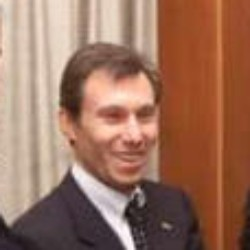
\includegraphics[scale=0.5]{Imagens/exemplo_flip_01}
		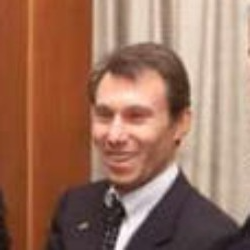
\includegraphics[scale=0.5]{Imagens/exemplo_flip_02}
	\end{center}
	\caption {\label{exemplo_flip_lfw}Exemplo de uma imagem e sua versão com \textit{flip}} \legend {Fonte: LFW} %Colocar fonte do LFW
\end{figure}
% TODO: DETALHAR

% Para gerar as estatísticas de modelo, foi calculada a precisão e acurácia de cada um, junto com o seu tempo de
% inferência. Onde

\section{\textit{Datasets}}\label{sec_datasets}
Nessa seção serão apresentados os dois \textit{datasets} utilizados, \textit{Labeled Faces in the Wild} (LFW),
que foi utilizado para o treinamento dos modelos, e Faces - UFS, que foi utilizado para a validação dos modelos.

\subsection{\textit{Labeled Faces in the Wild}}
Este \textit{dataset} possui imagens da face de várias celebridades, classificadas com o nome da pessoa.
Para esse trabalho, foi utilizada uma variação do LFW, que agrupa as imagens em triplas, \textbf{âncora},
\textbf{positiva} e \textbf{negativa}, para ser utilizado como dataset de treinamento, seguindo a técnica
de \textit{triplet distillation} \cite{triplet_distillation_face_recognition}.

Para realizar o treinamento do modelo, foi utilizada uma variação do \textit{dataset}
\textit{Labeled faces in the Wild} (LFW), que possui várias amostras contendo triplas com as imagens das faces,
assim facilitando o uso da técnica de \textit{triplet distillation} para o treinamento. Um exemplo pode ser visto
na \autoref{exemplo_dataset_lfw}.

\begin{figure}[htb]
	\begin{center}
		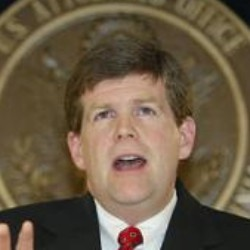
\includegraphics[scale=0.5]{Imagens/exemplo_triplet_01}
		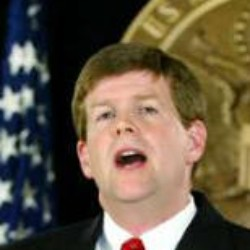
\includegraphics[scale=0.5]{Imagens/exemplo_triplet_02}
		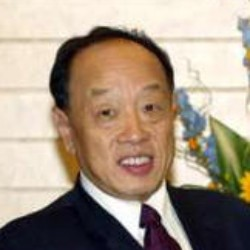
\includegraphics[scale=0.5]{Imagens/exemplo_triplet_03}
	\end{center}
	\caption{\label{exemplo_dataset_lfw}Exemplo de triplas do LFW}
	\legend {Fonte: LFW}
\end{figure}

\subsection{Faces - UFS}\label{subsec_dataset_faces_ufs}
Este \textit{dataset} possui faces coletadas de alunos da Universidade Federal de Sergipe (UFS) \cite{leandro}.
Para coletar essas imagens, foi disponibilizado um estande com uma câmera, monitor, teclado e mouse, permitindo
que qualquer pessoa pudesse salvar uma imagem com o seu nome.

Esse \textit{dataset} foi utilizado na etapa de validação do modelo (\ref{sec_avaliacao_modelo}), por apresentar faces
novas e com um padrão diferente do LFW, já que o seu público consiste em celebridades, principalmente dos Estados
Unidos. Enquanto o \textit{dataset} coletado na UFS possui um público diferente, estudantes ou funcionários da UFS.

\section{Resultados}\label{sec_resultados}
Para obter os resultados, primeiro foram definidas as métricas que serão usadas para avaliar os modelos. Em seguida,
cada modelo foi submetido ao método de avaliação escolhido (\autoref{sec_avaliacao_modelo}), com o objetivo de
validar e comparar o desempenho na tarefa de reconhecimento facial de cada um, junto com o seu tempo de execução.

Para realizar a avaliação na tarefa de reconhecimento facial, os modelos foram executados em um computador, com um
AMD Ryzen 5 4600G, com seis núcleos, clock máximo de 4.2GHz, 16GB de memória RAM e arquitetura x86 64,
e em um Raspberry Model B um processador com quatro núcleos, clock de 1.GHz, 1GB de memória RAM e arquitetura armv7l,
de 32 bits.
Na etapa de avaliação de performance em microcontroladores, foi utilizado
o ESP32-S3 N16R8, descrito na \autoref{sec_dispositivo}.

\subsection{Métricas usadas}\label{sect_restultados_metricas}
Para avaliar o desempenho, foram utilizadas as métricas de precisão (\ref{sect_restultados_metricas_precisao})
e acurácia (\ref{sect_restultados_metricas_acuracia}). Como a avaliação é binária, a imagem prevista é a imagem
verdadeira, também foi utilizada a matriz de confusão, para facilitar o entendimento dos acertos e erros, quanto
facilitar o cálculo da precisão e acurácia.

\label{sect_restultados_metricas_precisao}
A precisão pode ser calculada pela \autoref{eq_precisao} e a acurácia pela \autoref{eq_acuracia}.
Onde a variável $TP$ indica o valor que foi previsto corretamente como verdadeiro, enquanto a variável $FP$ indica o
valor que foi previsto falsamente como verdadeiro.
Considerando o método de avaliação utilizada, a variável $TP$ indica os casos onde o modelo escolheu corretamente a
imagem, e a variável $FP$  indica quando o modelo escolheu a imagem errada.

\begin{equation}\label{eq_precisao}
	\text{Precisão} = \frac {TP} {TP + FP}
\end{equation}

\label{sect_restultados_metricas_acuracia}
\begin{equation}\label{eq_acuracia}
	\text{Acurácia} = \frac {TP + TN} {TP + TN + FP + FN}
\end{equation}

\subsection{Avaliação do modelo}
Para a avaliação do modelo, o método descrito na \autoref{sec_avaliacao_modelo} foi executado 10 vezes,
utilizando o \textit{dataset} Faces - UFS (\ref{subsec_dataset_faces_ufs}), medindo o tempo médio de inferência,
desvio padrão e acurácia de cada execução.
Com isso, esses resultados, foi gerada a \autoref{acuracia_tempo_inferencia_modelos_desktop}, onde as
métricas são dos modelos descritos na \autoref{sec_modelo_utilizado}.


\begin{table}[htb]
\centering
\ABNTEXfontereduzida
\caption[Acurácia e tempo de inferência com o dataset Faces - UFS (Desktop)]{Acurácia e tempo de inferência com o dataset Faces - UFS (Desktop)}
\label{acuracia_tempo_inferencia_modelos_desktop}
\begin{tabular}{ |c|c|c|c|c| }
	\hline
	\textbf{Modelo} & \textbf{Quantização} & \textbf{Acurácia (\%)} & \textbf{Tempo médio de inferência (ms)} & \textbf{Método de treinamento} \\
	\hline
	MobileFaceNet 	&-	& 	100.00  & $129 \pm 2.002$ & Pré-treinado + \textit{Triplet Loss} \\
	MobileFaceNet 	&uint8	& 	100.00  & $443 \pm 2.734$ & Pré-treinado + \textit{Triplet Loss} \\
	Rafael-2	&-	& 	 3.25 & $115 \pm 0.553$ & \textit{Triplet Distillation} \\
	Rafael-2	&uint8	& 	 24.03& $103 \pm 0.209$ & \textit{Triplet Distillation} \\
	MobileNetV3Small&-	& 	 7.14& $37 \pm 0.701$ & \textit{Triplet Distillation} \\
	\hline
\end{tabular}
\legend{Fonte: Autor}
\end{table}

A \autoref{acuracia_tempo_inferencia_modelos_desktop} contém os resultados dos testes feitos com os modelos
MobileFaceNet, Rafael-2 e MobileNetV3Small, mostrando o tipo de quantização que foi feito, acurácia, tempo
médio de inferência e o método de treinamento.

Com isso, é possível notar que o modelo que o melhor modelo foi o MobileFaceNet, por conta da sua estrutura
mais robusta que tem o foco na tarefa de reconhecimento facial. Além disso, fica evidente a diferença entre
o tempo de inferência do MobileFaceNet quantizado e não quantizado, isso se deve pelo ambiente de execução
do TensorFlowLite, que em tempo de execução converte os pesos quantizados de inteiro de 8 bits para float.


\begin{table}[htb]
\centering
\ABNTEXfontereduzida
\caption[Acurácia e tempo de inferência com o dataset Faces - UFS (Raspberry Pi Model B)]{Acurácia e tempo de inferência com o dataset Faces - UFS (Raspberry Pi Model B)}
\label{acuracia_tempo_inferencia_modelos_raspberry}
\begin{tabular}{ |c|c|c|c|c| }
	\hline
	\textbf{Modelo} & \textbf{Quantização} & \textbf{Acurácia (\%)} & \textbf{Tempo médio de inferência (ms)} & \textbf{Método de treinamento} \\
	\hline
	MobileFaceNet 	&-	& 	100.00  & $3677 \pm 13.218$ & Pré-treinado + \textit{Triplet Loss} \\
	MobileFaceNet 	&uint8	& 	 99.35  & $10607 \pm 28.274$ & Pré-treinado + \textit{Triplet Loss} \\
	Rafael-2	&-	& 	 3.25 	& $1779 \pm 10.346$ & \textit{Triplet Distillation} \\
	Rafael-2	&uint8	& 	 24.03	& $2515 \pm 10.8334$ & \textit{Triplet Distillation} \\
	\hline
\end{tabular}
\legend{Fonte: Autor}
\end{table}

A \autoref{acuracia_tempo_inferencia_modelos_raspberry} contém os resultados dos experimentos feitos no
Raspberry Pi Model B, utilizando o \textit{dataset} Faces - UFS e o interpretador do tflite-runtime
\footnote{Disponível em: \url{https://pypi.org/project/tflite-runtime/}. Acessado em Maio 2025.}
no lugar do interpretador do tensorflow, por ser a versão indicada para executar modelos de aprendizagem de
máquina em dispositivos embarcados, móveis ou com baixo poder computacional. Por conta de uma limitação
do tflite-runtime, o modelo MobileNetV3Small não foi incluído nos testes.

Com isso, é possível observar que os resultados são parecidos com o experimento no Desktop, o MobileFaceNet
permanece com acurácia alta, com e sem quantização. A diferença no tempo de execução entre os tipos de
quantização também é parecida, por conta da forma como o \textit{runtime} lida com a quantização do modelo.

\begin{table}[htb]
\centering
\ABNTEXfontereduzida
\caption[Acurácia e tempo de inferência (ESP)]{Acurácia e tempo de inferência Faces - UFS (ESP)}
\label{acuracia_tempo_inferencia_modelos_esp}
\begin{tabular}{ |c|c|c|c|c| }
	\hline
	\textbf{Modelo} & \textbf{Quantização} & \textbf{Acurácia (\%)} & \textbf{Tempo médio de inferência (ms)} & \textbf{\textit{Runs}} \\
	\hline
	MobileFaceNet 	&uint8	& 	93.33& $3703 \pm 0.6010$ & 5 \\
	MobileFaceNet 	&uint8	& 	93.33& $3703 \pm 0.6067$ & 10 \\
	Rafael-2	&uint8	& 	93.33& $737 \pm 0.061$ & 5\\
	Rafael-2	&uint8	& 	93.33& $737 \pm 0.056$ & 10\\
	\hline
\end{tabular}
\legend{Fonte: Autor}
\end{table}

A \autoref{acuracia_tempo_inferencia_modelos_esp} mostra o resultado dos testes feitos no ESP32-S3,
utilizando a ferramenta idf.py\footnote{Disponível em:
\url{https://docs.espressif.com/projects/esp-idf/en/stable/esp32/api-guides/tools/idf-py.html}.
Acessado em Maio 2025.}
com a biblioteca Tensorflow Lite Micro\footnote{Disponível em: \url{
https://github.com/espressif/esp-tflite-micro}. Acessado em Maio 2025.},
e com uma versão com uma versão limitada do \textit{dataset} Faces - UFS, contendo apenas três imagens.
O foco desse experimento foi o medir o tempo de inferência dos modelos e avaliar a sua acurácia
no ESP32-S3, onde foi possível perceber os limites do do microcontrolador.

Com isso, é possível observar que acurácia permanece igual, isso é causado pela limitação na
quantidade de imagens utilizada, visto que a memória do ESP32-S3 é limitada, então não possível
portar todo \textit{dataset} utilizado no experimento da tabela
\autoref{acuracia_tempo_inferencia_modelos_desktop}.

% Pode-se observar que, na \autoref{acuracia_tempo_inferencia_modelos_esp}, a acurácia do modelo se manteve
% a mesma.

\section{Conclusão}
Neste capítulo, foi possível descrever melhor os pontos fortes e fracos do ESP32-S3 N16R8, que foi o microcontrolador
alvo para embarcar o modelo de reconhecimento facial. Além disso, foi possível destacar os modelos, suas técnicas de
treinamento e validação, junto com os \textit{datasets} utilizados durante o experimento. Também, foi possível demonstrar
os resultados dos experimentos, junto com as suas métricas e dispositivos utilizados, junto com a comparação dos seus
resultados, onde esses dispositivos são o Desktop, Raspberry Pi e ESP32-S3.
